\section{Concept: flexures}
\label{Concept: flexures}
The second concept is fully based on flexure mechanisms. First the options to obtain a translational motion are discussed, thereafter the solutions to obtain a rotational motion. Next three concepts are discussed and finally a concept is chosen and elaborated in more detail in section \ref{Sec: Final design}.    
\subsection{Degrees of freedom }
\subsubsection{Translational degrees of freedom}
As mentioned in section \ref{sec:requirements} the system has to have three translational degrees of freedom. In table \ref{tab:transsolutions} three options are shown to obtain a translational motion by only making use of flexures. Moreover both the advantages and disadvantages are shown.

\begin{table}[h]
\caption{Flexure based translational solutions}
\label{Tab: flexure translational}
\begin{tabular}{p{4cm}|p{4cm}p{4cm}p{4cm}}
Translational solution   & Leaf spring \cite{lecturesheets} &  \cite{PrecisionParallel} & Flexures \cite{lecturesheets} \\ \hline
Figure for clarification &     
    \begin{minipage}{4cm}
      \includegraphics[width=\linewidth]{images/}
    \end{minipage} 
    &     
    \begin{minipage}{4cm}
      \includegraphics[width=\linewidth]{images/}
    \end{minipage} 
    &     
    \begin{minipage}{4cm}
      \includegraphics[width=\linewidth]{images/}
    \end{minipage} \\ \hline
Advantages               & No parasitic motion and larger range compared to single leaf spring system     & Easier to manufacture compared to double leaf spring system  & Easy to manufacture and easy to analyse stiffness and displacement \\ \hline
Disadvantages            &  Less stiffness in the constrained direction compared to single leaf spring system                      & The system will have a parasitic motion.   & Less stiffness in direction of constrains, moreover the flexures will relative easy bend and buckle \\ 
\end{tabular}
\end{table}


\subsubsection{Rotational degrees of freedom}
Since the flexure based designs have three translational degrees of freedom the system
The design has to have two rotational degrees of freedom, one of 45$^{\circ}$ and one of 90$^{\circ}$. In this section several solutions for one rotational degree of freedom are shown.

\begin{table}[h]
\caption{Flexure based rotational solutions}
\label{Tab: flexure rotational}
\begin{tabular}{p{4cm}|p{4cm}p{4cm}p{4cm}}
Rotational solution   &  Curved flexure \cite{BrouwerELASTICDEFLECTION}   & Cross Flexure pivot \cite{Dearden2018CylindricalPivots} & Flex-16 Hinge \cite{Fowler2014Flex-16:Citation} \\ \hline
Figure for clarification &     
    \begin{minipage}{4cm}
      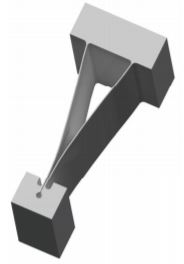
\includegraphics[width=\linewidth]{images/Cross_Brouwer.JPG}
    \end{minipage} 
    &     
    \begin{minipage}{4cm}
      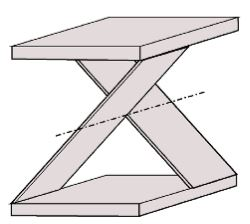
\includegraphics[width=\linewidth]{images/Cross_Flexure.JPG}
    \end{minipage} 
    &     
    \begin{minipage}{4cm}
      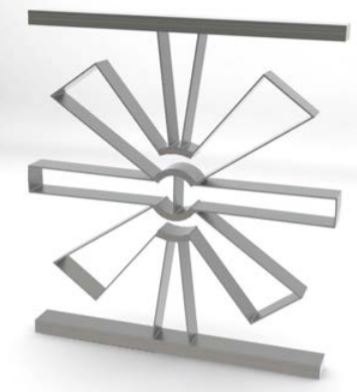
\includegraphics[width=\linewidth]{images/Flex16.JPG}
    \end{minipage} \\ \hline
Maximum rotation      & 45$^o$ &  45$^o$ & 90$^o$  \\ \hline
Advantages           &  2.5 to 14 times stiffer in stiff 
direction compared to single leaf-spring & No need of lubrication. Neither
wear nor friction occurs \cite{Haringx1949TheElement}.  & Is able to rotate 
over 90 degrees and it is a monolithic and compact design\\ \hline
Disadvantages            &  Large rotation results in limited stiffness reduction and hard to manufacture & Buckling may occur when heavily loaded, also large rotations results in a small displacement of the pivot point \cite{Haringx1949TheElement}.  & Low off-axis  stiffnesses leads to vibration problems  \\ 
\end{tabular}
\end{table}

The second concept is based on flexures, as mentioned in section \ref{requirementandassumptions} the system has four degrees of freedom, two translations and two rotations. 

To obtain a rotation of 45 degrees around the y axis, a cross-axis flexural pivot is used. Furthermore the rotation of 90 degrees around the z axis is obtained by making use of the Flex-16 hinge \cite{Fowler2014Flex-16:Citation}. Both the translations in the x and z directions are performed by double leaf spring intermediate body system, since the system has to translate over a relatively large range and has no parasitic motion. 

\subsection{Concepts evaluation}

\subsubsection{Concept A}

\subsubsection{Concept B}

\subsubsection{Concept C}

\subsection{Concept selection}